
\section{Spontaneous Symmetry Breaking and Mass (Weinberg, 1967)}
%
In summary of the situation thus far, the Lagrangian is made up of a $\psi$ kinetic term, a vector boson kinetic term, a $\psi$ mass term and a vector boson mass term:
\begin{equation}
\mathcal{L} = \mathcal{L}_D + \mathcal{L}_{YM} + \mathcal{L}_m + \mathcal{L}_M,
\end{equation}
where the first two terms are SU(2)$_L \otimes$U(1)$_Y$ gauge invariant, and the
second two break the symmetry: the problems are all to do with the mass terms.
\begin{equation}
\mathcal{L}_m = m(\bar{\psi}_L \psi_R + \bar{\psi}_R \psi_L) + ...
\end{equation}
breaks SU(2)$_L \otimes$U(1)$_Y$ explicitly, due to chirality, and
\begin{equation}
\mathcal{L}_M = m_W^2W_\mu^\dagger W^\mu + \frac{1}{2}m_Z^2 Z_\mu Z^\mu 
\end{equation}
also breaks SU(2)$_L \otimes$U(1)$_Y$ explicitly: $Z_\mu \neq W_\mu^3$ and $m_z \neq m_W$. We have Weinberg mixing, which again is due to chirality. 

Soft breaking of global symmetries is OK, but gauge symmetries must be exact so that the Noether current is conserved. Otherwise you miscount the degrees of freedom.
%
\subsection{Lepton Masses}
%
Under SU(2)$_L$:
\begin{equation}
\psi_L \to U \psi_L \qquad \text{and} \qquad \psi_R \to \psi_R, \qquad \text{where} \qquad U=\exp\bigg(\frac{i}{2}\underline{\alpha}\cdot\underline{\tau}\bigg);
\end{equation}
and under U(1)$_Y$:
\begin{equation}
\psi_L \to \exp\bigg(-\frac{i}{2}\beta\bigg) \psi_L \qquad \text{and} \qquad \psi_R \to \psi_R.
\end{equation}
An invariant mass term in SU(2)$_L \otimes$U(1)$_Y$ is impossible. But what about a Yukawa term ($\phi \bar{\psi} \psi$)? For this we need a scalar field, $\phi$. The simplest way to do this (but not the only way!) is to introduce a spin zero complex scalar doublet,
\[\phi = \left( \begin{array}{cc}
\phi^+ \\
\phi^0
\end{array} \right), \]
such that under SU(2)$_L$, $\phi \to U \phi$ (i.e. a doublet) and under U(1)$_Y$ $\phi \to \exp(i \beta /2)$ (i.e. $Y$ = 1/2). Then the additional Yukawa term in the Lagrangian looks like
\begin{equation}
\mathcal{L}_Y = -y_\psi(\bar{\psi}_L \phi \psi_R + \bar{\psi}_R \phi^\dagger \psi_L).
\end{equation}
This term is invariant because 
\begin{equation}
\bar{\psi}_L \phi \psi_R \to
\begin{cases}
\bar{\psi}_L U^\dagger U \phi \psi_R \qquad \qquad= \bar{\psi}_L \phi \psi_R \qquad \text{under SU(2)}_L,\\
\bar{\psi}_L e^{i \beta/2} e^{i \beta/2} \phi e^{-i\beta} \psi_R =\bar{\psi}_L \phi \psi_R \qquad \text{under U(1)}_Y.
\end{cases}
\end{equation}
Note that
\[ Q \qquad = \qquad T_3 \qquad + \qquad Y: \]
\[\left( \begin{array}{cc}
1 & 0  \\
0 & 0  \end{array} \right)=
\left( \begin{array}{cc}
1/2 & 0  \\
0 & -1/2  \end{array} \right) +
\left( \begin{array}{cc}
1/2 & 0  \\
0 & 1/2  \end{array} \right), \]
so $\phi^+$ has $Q = +1$ and $\phi^0$ has $Q=0$ (how fortuitous). Since $\phi^\dagger \phi$ is SU(2)$_L \otimes$U(1)$_Y$ invariant,
\begin{equation}
\mathcal{L}_\phi = \partial_\mu \phi^\dagger \partial^\mu \phi - V(\phi^\dagger \phi)
\end{equation}
has the correct global symmetry.

We still have no fermion masses. But because $\phi^0$ has $Q=0$ we can have spontaneous symmetry breaking. Choose a form for the potential
\begin{equation}
V(\phi^\dagger \phi) = \lambda \bigg(\phi^\dagger \phi - \frac{1}{2}v^2\bigg)^2.
\end{equation}
The minimum of $V$ is when $\phi^\dagger \phi = v^2/2$, so it's helpful to pick 
\[\phi^0 = \frac{1}{\sqrt{2}} = \left( \begin{array}{cc}
0   \\
v   \end{array} \right). \]
We can make this choice without loss of generality, due to global symmetry: we could have chosen e.g.
\[\phi^0 = u_0\frac{1}{\sqrt{2}} = \left( \begin{array}{cc}
0   \\
v   \end{array} \right), \]
but then let $\psi_L \to u_0 \psi_L$ and $\mathcal{W}_\mu \to u_0 \mathcal{W}_\mu u_0^\dagger$, and the Lagrangian would be unchanged.
Note that $i \underline{\alpha}\cdot \underline{T} \phi^0 \neq 0$, $i\beta\phi^0/2 \neq 0$, so both SU(2)$_L$ and U(1)$_Y$ are broken. But $Q\phi^0 = 0$ so U(1)$_Q$ remains unbroken. In other words SU(2)$_L$ $\otimes$U(1)$_Y$ $\to$ U(1)$_Q$. If we set $\phi \to \phi^0$ in $\mathcal{L}_Y$,
\begin{equation}
\mathcal{L}_Y \to -y_\psi (\bar{\psi}_L \phi_0 \psi_R + \bar{\psi_R} \phi_0^\dagger \psi_L) = -\frac{yv}{\sqrt{2}}(\bar{\psi}_L \psi_R + \bar{\psi}_R \psi_L) = -m_\psi \bar{\psi} \psi,
\end{equation}
i.e. we end up with the usual Dirac mass, where $m_\psi = y_\psi v/\sqrt{2}$, and is different for each of the leptons, dependent on their individual Yukawa couplings. The neutrinos remain massless. 

The only freedom is in the choice of $v$, which sets the scale, and in the parameters $y_e, y_\mu, y_\tau$ which fix the lepton masses.

Expanding around the minimum,
\[\phi = \phi^0 + \chi = \frac{1}{\sqrt{2}} \left( \begin{array}{cc}
\chi_1 + i \chi_2  \\
v + h + i \chi_3  \end{array} \right), \]
then 
\begin{equation}
\partial_\mu \phi^\dagger \partial^\mu \phi = \frac{1}{2} (\partial_\mu h)^2 + \frac{1}{2} (\partial_\mu \underline{\chi})^2, \qquad \text{where } \underline{\chi} = \chi_i; \ i=1,2,3.
\end{equation}
But
\begin{equation}
\phi^\dagger \phi -\frac{1}{2}v^2 = (\chi^\dagger \phi^0 + \phi^{\dagger 0}\chi) + \chi^\dagger \chi = vh + \frac{1}{2}h^2 + \frac{1}{2}\underline{\chi}^2,
\end{equation}
so 
\begin{equation}
V(\phi^\dagger \phi) = \lambda v^2 h^2 + \lambda v (h^3 + h \underline{\chi}^2) + \frac{\lambda}{4}(h^2 + \underline{\chi}^2)^2,
\end{equation}
so $h$ is massive: $m_h^2 = 2 \lambda v^2$, but the $\chi$ are massless: they are \textit{Goldstone} bosons. Because SU(2)$_L$ has dimension 3 and and U(1)$_Y$ and U(1)$_Q$ both have dimension 1, there are three Goldstone bosons because the degrees of freedom in the symmetry are reduced from 4 to 1 during symmetry breaking. $\lambda$ is a free parameter with a value $\approx 1/8$. 

Note that after spontaneous symmetry breaking we still have an SO(3) global symmetry, $\underline{\chi} \to R \underline{\chi}$, where $R^\dagger R =1$. This is called "custodial symmetry" or "custodial" SU(2) (because SO(3) $\cong$ SU(2)).

There are a number of vertices arising from the terms in $V$, which have the Feynman rules given in the figure.
\begin{figure}[!h]
  \centering
  \subfloat[3-point]{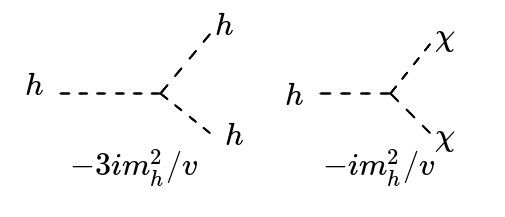
\includegraphics[width=0.5\textwidth]{figs/29a.png}}
  \hfill
  \subfloat[4-point]{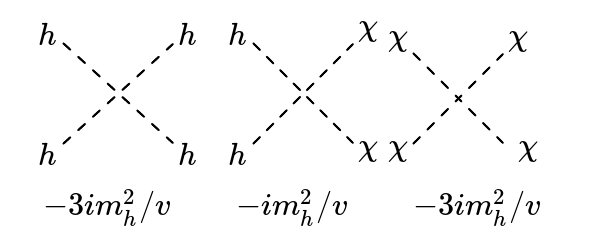
\includegraphics[width=0.5\textwidth]{figs/29b.png}}
\end{figure}
%
\subsection{Gauge Boson Masses}
%
$\mathcal{L}_\phi$ is invariant under \textit{global} SU(2)$_L \otimes$U(1)$_Y$. $\mathcal{L}_{YM}, \mathcal{L}_D$ and $\mathcal{L}_{Y}$ are all invariant under \textit{local} SU(2)$_L \otimes$U(1)$_Y$. So if we make $\mathcal{L}_\phi$ \textit{gauge} invariant, \textit{everything} will be gauge invariant! There is a unique prescription for achieving this:
\begin{equation}
\partial_\mu \phi \to \mathcal{D}_\mu \phi = (\partial_\mu - ig \mathcal{W}_\mu - \frac{1}{2} ig^\prime B_\mu) \phi,
\end{equation}
since $\phi$ is an SU(2) doublet, with $Y = +1/2$, and
\begin{equation}
\mathcal{L}_\phi \to \mathcal{L}_h = (\mathcal{D}_\mu \phi)^\dagger \mathcal{D}_\mu \phi - V(\phi^\dagger \phi).
\end{equation}
Now after spontaneous symmetry breaking, $\phi \to \phi^0 + \chi$, where $\partial_\mu \phi^0 = 0$. So
\begin{equation}
\begin{split}
\mathcal{D}_\mu \phi^0 &= -ig \underline{W}_\mu \cdot \underline{T}_\mu \phi^0 - \frac{1}{2} i g^\prime B_\mu \phi^0 \\
&= \frac{v}{2\sqrt{2}} 
\begin{pmatrix}  
-ig(W_\mu^1 - i W_\mu^2) \\
i(gW_\mu^3 - g^\prime B_\mu)
\end{pmatrix}, \\
\mathcal{D}_\mu \phi^{0 \dagger} \mathcal{D}^\mu \phi^0 &= \frac{v^2}{2} \bigg(\frac{g^2}{2} W_\mu^\dagger W^\mu + \frac{1}{4}(g W_\mu^3 - g^\prime B_\mu)^2 \bigg).
\end{split}
\end{equation}
So $m_W^2 = g^2v^2/4$, and $W$ becomes massive ($v \approx$ 50 GeV). $W_\mu^3$ and $B_\mu$ mix, but we know that already from the currents (because $j$ is not chiral).  
\[\left( \begin{array}{cc}
W^\mu_3 \\
B^\mu 
\end{array} \right) =
 \left( \begin{array}{cc}
\cos\theta_w & \sin\theta_w  \\
-\sin\theta_w & \cos\theta_w  \end{array} \right) 
\left( \begin{array}{cc}
Z^\mu \\
A^\mu 
\end{array} \right), \]
while $e = g \sin\theta_w = g^\prime \cos\theta_w$ so 
\begin{equation}
g W_\mu^3 - g^\prime B_\mu = \frac{g}{\cos \theta_w} (\cos\theta_w W_\mu^3 - \sin\theta_w B_\mu) = \frac{g}{\cos\theta} Z_\mu,
\end{equation}
and
\begin{equation}
\mathcal{D}_\mu \phi^{0 \dagger} \mathcal{D}^\mu \phi^0 = m_W^2 W_\mu^\dagger W^\mu + \frac{1}{2}m_Z^2 Z_\mu Z^\mu,
\end{equation}
with $m_Z^2 = g^2v^2/4\cos^2\theta_w = m_W^2/\cos^2\theta_w$, so $\rho = m_W^2/m_Z^2\cos^2\theta = 1$. $A_\mu$ remains massless, as expected, since U(1)$_Q$ is unbroken. So spontaneous symmetry breaking gives vector boson masses \textit{and} mixing.

There are also new interactions of vector bosons with scalars: $\phi = \phi^0 + \chi$, so
\begin{equation}
\mathcal{D}_\mu \phi^{\dagger} \mathcal{D}^\mu \phi = \mathcal{D}_\mu \phi^{0 \dagger} \mathcal{D}^\mu \phi^0 + \mathcal{D}_\mu \chi^{\dagger} \mathcal{D}^\mu \phi^0 + \mathcal{D}_\mu \phi^{0 \dagger} \mathcal{D}^\mu \chi + \mathcal{D}_\mu \chi^{\dagger} \mathcal{D}^\mu \chi,
\end{equation}
which leads to the mixing terms
\begin{equation}
ig(\phi^{0 \dagger} \underline{T} \partial_\mu \chi -\partial_\mu \chi^\dagger \underline{T} \phi^0) \cdot \underline{W}^\mu + i g^\prime (\phi^{0 \dagger} \partial_\mu \chi - \partial_\mu \chi^\dagger \phi^0) B^\mu.
\end{equation}
To simplify this, write $A_\mu^a = (W_\mu^i, B_\mu)$, $\tilde{T}^a = (gT^i, g^{\prime Y}) = (g\sigma^i/2, g^\prime/2)$, so that the mixing is
\begin{equation}
+i(\phi^{0 \dagger} \tilde{T}^a \partial_\mu \chi - \partial_\mu \chi^\dagger \tilde{T}^a \phi^0)A^{\mu a} = +i \tilde{J}_\mu^a A^{\mu a}.
\end{equation}
$\tilde{J}_\mu^a$ is actually the linear part of the Noether current of the SU(2)$_L \otimes$U(1)$_Y$ symmetry. In terms of real fields, writing 
\[\phi^0 = \frac{1}{\sqrt{2}} \left( \begin{array}{cc}
0 \\
v
\end{array} \right); \qquad
\chi = \frac{1}{\sqrt{2}}
 \left( \begin{array}{cc}
\chi_1 + i \chi_2 \\
h + i \chi_3  \end{array} \right), \]
it is easy to show (left as an exercise) that
\begin{equation}
\tilde{J}_\mu^a = -i F^{T a}_i \partial_\mu \chi_i = -i \partial_\mu \chi_i^T F_i^a,
\end{equation}
where
\[F_i^a = \frac{v}{2} \left( \begin{array}{cccc}
0 & -g & 0 & 0 \\
-g & 0 & 0 & 0 \\
0 & 0 & g & -g^\prime 
\end{array} \right). \]
So the mixing is between the vector bosons $A_\mu^a$ and the Goldstone bosons $\chi_i$ (\textit{not} the Higgs boson $h$): the mixing term is $A_\mu^a F^{a T} \partial_\mu \chi$. Note that
\begin{equation}
<0|\tilde{J}_\mu^a|\chi_i> = p_\mu F^a_i,
\end{equation}
so $F_i^a$ are the decay constants of the Goldstone bosons. $\partial^\mu \tilde{J}_\mu^a = 0 \implies p^2=0$ (i.e. the Goldstone bosons are massless: this is another derivation of Goldstone's theorem). It is easy to see that "$F^a = \tilde{T}^a \phi^0$ is the basis for the Goldstone bosons.

The mass term of the vector bosons is given by
\begin{equation}
\begin{split}
\mathcal{D}_\mu \phi^{0 \dagger} \mathcal{D}^\mu \phi^0 &= \frac{1}{2} \phi^{0 \dagger} \tilde{T}^a \tilde{T}^b \phi^0 A_\mu^a A^{\mu b} \\
&= \frac{1}{2}(F^TF)^{ab} A_\mu^a A^{\mu b}.
\end{split}
\end{equation}
In components,
\[(F^TF)^{ab} = \frac{v^2}{4} \left( \begin{array}{cccc}
g^2 & 0 & 0 & 0 \\
0 & g^2 & 0 & 0 \\
0 & 0 & g^2 & -gg^\prime \\
0 & 0 & - gg^\prime & g^{\prime 2} 
\end{array} \right), \]
with two $g^2v^2/4$ eigenvalues corresponding to $W^\pm$, one $(g^2 + g^{\prime 2})v^2/4$ eigenvalue corresponding to $Z$, and one $0$ eigenvalue corresponding to $\gamma$.

The equality of the first three diagonal elements is due to the SO(3) custodial symmetry, and ensures that the Veltman parameter
\begin{equation}
\rho = \frac{m_W^2}{m_Z^2 \cos^2\theta_w} = 1.
\end{equation}
%
\subsection{Unitarity Gauge}
%
As we now have a gauge theory, we need to fix a gauge (just as in QED): the degrees of freedom due to gauge transformations are not physical. One way to do this is to notice that the Goldstone bosons arise because of the SU(2)$_L \otimes$U(1)$_Y$ symmetry: for $\underline{\alpha}, \chi$ small, 
\begin{equation}
\begin{split}
&\text{SU(2)}_L: \quad U\phi \sim \phi^0 + i\underline{\alpha}\cdot \underline{T} \phi^0 + \chi = \frac{1}{\sqrt{2}} \bigg[ 
\begin{pmatrix}
0 \\ v
\end{pmatrix}
+ \frac{v}{2}
\begin{pmatrix}
(\alpha_2 + i \alpha_1) \\ -i\alpha_3
\end{pmatrix}
+ \begin{pmatrix}
\chi_1 + i \chi_2 \\ h + i \chi_3
\end{pmatrix} \bigg] \\
&\text{U(1)}_Y: \quad e^{i\beta /2}\phi \sim \phi^0 + i\frac{\beta}{2}\phi^0 + \chi = \frac{1}{\sqrt{2}} \bigg[ 
\begin{pmatrix}
0 \\ v
\end{pmatrix}
+ \frac{v}{2}
\begin{pmatrix}
0 \\ i\beta
\end{pmatrix}
+ \begin{pmatrix}
\chi_1 + i \chi_2 \\ h + i \chi_3
\end{pmatrix} \bigg],
\end{split}
\end{equation}
so we can eliminate $\chi_1, \chi_2, \chi_3$ just by choosing $\alpha_1, \alpha_2, \alpha_3, \beta$. Note that we cannot eliminate $h$: $\alpha_3 + \beta$ has no effect, since
\begin{equation}
Q \phi^0 = (T_3 + Y) \phi^0 = 0:
\end{equation}
U(1)$_Q$ is unbroken.

This is equivalent to adopting gauge fixing conditions for the broken symmetries:
\begin{equation}
\begin{split}
\chi^\dagger \underline{T} \phi^0 - \phi^{0 \dagger} \underline{T} \chi &= 0 \\
\chi^\dagger \phi^0 - \phi^{0 \dagger} \chi &= 0,
\end{split}
\end{equation}
i.e. $F_i^T\chi_i=0 \implies \chi_i=0$. With these conditions, the mixing terms between vector bosons and Goldstone bosons disappear, and we can write
\[\phi = \frac{1}{\sqrt{2}} = \left( \begin{array}{cc}
0   \\
v + h  \end{array} \right). \]
Substituting into the Lagrangian, 
\begin{equation}
\begin{split}
\mathcal{L}_h &= (\mathcal{D}_\mu \phi)^\dagger \mathcal{D}^\mu \phi - V(\phi^\dagger \phi) \\
&= \frac{1}{2}(\partial_\mu h)^2 - \frac{1}{4}(2vh + h^2)^2 + g^2(v+h)^2 \bigg(\frac{1}{4} W_\mu^\dagger W_\mu + \frac{1}{8\cos^2\theta_w} Z_\mu Z^\mu \bigg) \\
&= \frac{1}{2}(\partial_\mu h)^2 -\frac{1}{2}m_h^2h^2\bigg(1 + \frac{h}{v}\bigg)^2 + \bigg(1+ \frac{2h}{v} + \frac{h^2}{v^2}\bigg)\bigg(m_W^2 W_\mu^\dagger W^\mu + \frac{1}{2}m_Z^2 Z_\mu Z^\mu\bigg), \\
\mathcal{L}_Y &= -\sum_{gen} y(v+h)\bar{\psi}\psi \\
&= -\sum_{gen} m_\psi \bigg(1 +\frac{h}{v}\bigg)\bar{\psi}\psi.
\end{split}
\end{equation}
When added to $\mathcal{L}_{YM} + \mathcal{L}_D$, this gives the electroweak sector in unitary gauge.
\textbf{Note:}
\begin{enumerate}
\item this is precisely our previous theory with the addition of the Higgs;
\item all masses are due to spontaneous symmetry breaking, i.e. they are proportional to $v$;
\item all (massive) particles couple to the Higgs, including itself, with couplings to their mass in units of $v$.
\end{enumerate}
  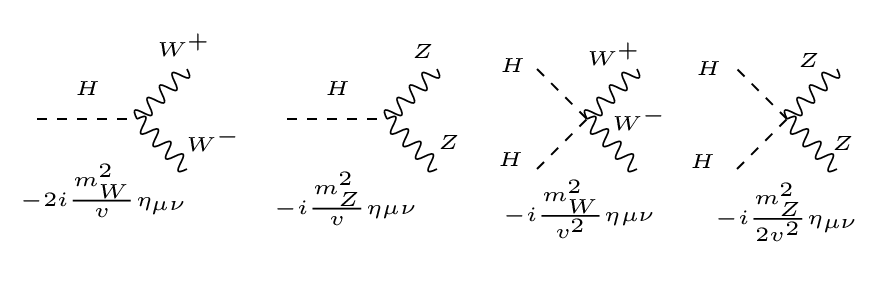
\includegraphics[width=\linewidth]{figs/31a.png}
  %
\subsection{Unitarity (in the unitary gauge)}
%
Consider the process $W_L^+ W_L^- \to W_L^+ W_L^-$ for $E \gg m_W$.
\newline
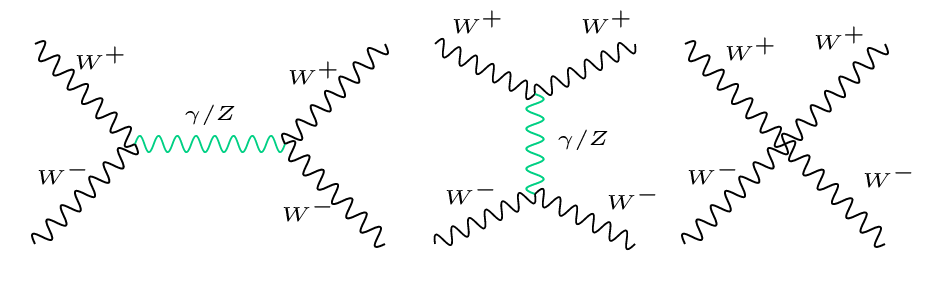
\includegraphics[width=\linewidth]{figs/32a.png}
Each of these diagrams goes like $\sim (E/m_W)^4$. Added together, the leading singularities cancel: after a long and difficult calculation, using $\epsilon_\mu^L = k_\mu/m + \mathcal{O}(m/k)$ and including the higher order terms, you find
\begin{equation}
\mathcal{M} = \frac{-ig^2}{4m_W^2}u \sim\bigg(\frac{E}{m_W}\bigg)^2.
\end{equation}
For unitarity to be retained, we also need to include the Higgs contributions.
\newline
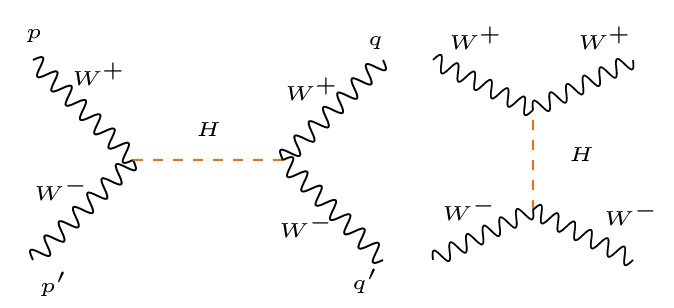
\includegraphics[width=\linewidth]{figs/32b.png}
\begin{equation}
\begin{split}
\mathcal{M}_h &= \bigg(-\frac{2im_W^2}{v}\bigg)^2\bigg(\frac{p \cdot p^\prime}{m_W^2} \frac{i}{(p+p^\prime)^2 -  m_h^2}\frac{q \cdot q^\prime}{m_W^2} + \frac{p \cdot q}{m_W^2} \frac{i}{(p-q)^2 - m_h^2}\frac{p^\prime \cdot q^\prime}{m_W^2} \bigg) \\
&= -\frac{ig^2}{4m_W^2} \bigg( \frac{(s-2m_W^2)^2}{s-m_h^2} + \frac{(t-2m_W^2)^2}{t-m_h^2} \bigg) \\
&\approx -\frac{ig^2}{4m_W^2} \bigg(s + t + \mathcal{O}\bigg(\frac{1}{s}, \frac{1}{t} \bigg) \bigg) \\
&\approx + \frac{ig^2}{4m_W^2}u,
\end{split}
\end{equation}
where we have used $s + t + u = 4m_W^2$. This cancels the contribution from the $\gamma, Z$ exchange above. So unitarity is preserved for $E \gg m_W$. This is a reflection of the gauge invariance.

It is easy to see that:
\begin{enumerate}
\item processes with no Higgs diagram (e.g. $\nu\bar{\nu} \to W^+ W^-$) are unitarity without the Higgs;
\item processes with a Higgs diagram (e.g. $W^+W^- \to W^+W^-$) need the Higgs for unitarity;
\item for processes with four vector bosons, computing the unitary cross section can be very difficult as cancellations can be delicate (see later).
\end{enumerate}
%
\subsection{Renormalisability ('t Hooft, 1971)}
% 
Our Lagrangian $\mathcal{L}_{YM} + \mathcal{L}_D + \mathcal{L}_Y + \mathcal{L}_h$ is fully gauge invariant under SU(2)$_L \otimes$U(1)$_Y$. Spontaneous symmetry breaking chooses the vacuum, but does not break gauge invariance. We need gauge fixing to absor the redundant degrees of freedom. For example, in electromagnetism, we require a choice such as the Lorentz gauge condition $\partial_\mu A^\mu = 0$. We can do this either by hand, or by using a Lagrange multiplier:
\begin{equation}
\mathcal{L} = - \frac{1}{4}F_{\mu \nu}F^{\mu \nu} - \frac{1}{2\xi}({\partial_\mu A^\mu})^2,
\end{equation}
where the second term is the gauge fixing term. Then the propagator becomes
\begin{equation}
\Delta_{\mu \nu} = \frac{i}{k^2 _ i\epsilon}\bigg(-\eta_{\mu \nu} + (1-\xi)\frac{k_\mu k_\nu}{k^2} \bigg).
\end{equation}
Physical results such as cross sections must be independent of the gauge fixing parameter, $\xi$. This is because of gauge invariance, which implies Ward identities. For example, $\epsilon^\mu \mathcal{M}_\mu \implies k^\mu \mathcal{M}_\mu = 0$. For this to work, we need an \textit{exact} gauge symmetry (so $A_\mu$ couples to the conserved current, $j_\mu$: $\partial^\mu j_\mu =0$).

The clearest way of seeing this is through the path integral approach, which is necessary for non-abelian theories (see the QCD course). We write 
\begin{equation}
\mathcal{Z}[J] = \int\mathcal{D} A_\mu e^{iS[A,J]}, \qquad \text{where } S[A,J] = \int d^4x \bigg(-\frac{1}{4}\ tr F_{\mu \nu}F^{\mu \nu} - J_\mu^a A_\mu^a \bigg).
\end{equation}
Using the notation $A_\mu^\alpha = A_\mu - \partial_\mu \alpha$ to denote a gauge transformed field, we make an insertion of $\mathds{1}$ in the form
\begin{equation}
\mathds{1} = \int \mathcal{D}\alpha\ \delta ( G[A^\alpha]) det\bigg(\frac{\delta G}{\delta \alpha} \bigg),
\end{equation}
where $G[A^\alpha]$ are possible gauge-fixing conditions, e.g. for the Lorenz gauge $G[A^\alpha] = \partial_\mu A^{\alpha \mu}$. Making the change of variables $A_\mu \to A_\mu^\alpha$:
\begin{equation}
\mathcal{Z}[J] = \bigg( \int \mathcal{D}\alpha\ \delta ( G[A^\alpha]) det\bigg(\frac{\delta G}{\delta \alpha} \bigg)\bigg) \mathcal{D}A^\alpha_\mu e^{i S[A^\alpha,J]}.
\end{equation}
Gauge invariance implies $\mathcal{D}A_\mu^\alpha$ = $\mathcal{D}A_\mu$ and $S[A^\alpha, J] = S[A,J]$, so
\begin{equation}
\mathcal{Z}[J] = \bigg( \int \mathcal{D} \alpha \bigg) \int \mathcal{D} A_\mu \delta(G[A]) det \bigg(\frac{\delta G}{\delta \alpha} \bigg) e^{iS[A,J]}.
\end{equation}
$\int \mathcal{D} \alpha$ is now a decoupled factor which we can drop, as we will later be normalising the path integral. Now, considering a general gauge fixing condition $G[A] = -w(x)$ rather than $G[A] = 0$. We can investigate this by letting $G[A] \to G[A] + w(x)$ for some $w(x)$, then integrate over $w(x)$ with Gaussian weight $\exp(-i\int d^4x \ w(x)/2\xi)$. Then
\begin{equation}
\begin{split}
\mathcal{Z}[J] &= \int \mathcal{D} w\ \mathcal{D} A_\mu \ \delta(G[A] - w) det \bigg(\frac{\delta G}{\delta \alpha}\bigg) e^{i S [A,J]} e^{-i \int d^4x \frac{1}{2\xi}w^2} \\
&= \int \mathcal{D} A_\mu\ det\bigg(\frac{\delta G}{\delta \alpha}\bigg) e^{iS_\xi [A,J]} \\
\text{where } &S_\xi[A,J] = S[A,J] - \int d^4x\ \frac{1}{2\xi} (G[A])^2.
\end{split}
\end{equation}
In other words, this treatment is equivalent to the introduction of a Lagrange multiplier term into the Lagrangian, as discussed above.
For example, for QED in the Lorenz gauge, $G[A] = \partial_\mu A^\mu$. Then 
\begin{equation}
\frac{\delta G}{\delta \alpha} = -\partial^2,
\end{equation}
so $det(\delta G/\delta \alpha)$ is just an infinite constant, and we can ignore it. For a non-abelian gauge theory, $det(\delta G/\delta \alpha)$ is in general non-trivial, and we have to apply the Faddeev-Popov procedure, expressing the determinant as an exponential (see QCD course).

Note that if we take $\xi \to 0$, $G[A]=0$, which fixes the gauge. But if we take $\xi \to \infty$, $G[A]$ can be almost anything. However, physics is independent of $\xi$: a popular choice is $\xi =1$, the Feynman gauge.

In our spontaneously broken gauge theory we could also choose $G^a = \partial_\mu A^a$ for $a=1,2,3...$. But the gauge can also be fixed through Goldstone bosons: write
\begin{equation}
\mathcal{Z}[J]= \int \mathcal{D}A\ \mathcal{D}\chi\ det\bigg(\frac{\delta G}{\delta \alpha} \bigg) e^{i\int d^4x\ \mathcal{L}[A, \chi, J] - \frac{1}{2\xi}(G^a[A, \chi])^2}.
\end{equation}
One possible choice would be the unitary gauge: $\phi_i = 0$, i.e. $F^T\chi = 0$. However, a particularly clever choice is
\begin{equation}
G[A, \chi] = \partial^\mu A_\mu^a - \xi F^{a T}\chi,
\end{equation}
known as the $R_\xi$ gauges ('t Hooft, 1971). Then the gauge fixing term is
\begin{equation}
\begin{split}
\mathcal{L}_{GF} &= - \frac{1}{2\xi}(\partial^\mu A_\mu^a - \xi F^{a T}\chi)^2 \\
&= - \frac{1}{2 \xi}(\partial^\mu A_\mu^a)^2 - \frac{\xi}{2}(F^{a T}\chi)^2 + \partial^\mu A_\mu^a F^{a T}\chi.
\end{split}
\end{equation}
So we end up with quadratic terms for $A_\mu^a$ (the vector bosons) and $\chi$ (the Goldstone bosons):
\begin{equation}
\begin{split}
\mathcal{L}_{YM} &= -\frac{1}{4}(\partial_\mu A_\nu^a \partial^\mu A^{\nu a} - \partial_\mu A_\nu^a \partial^\nu A^{\mu a})^2, \\
\mathcal{L}_h &= + \frac{1}{2}A_\mu^a(F^TF)^{ab}A^{\mu b} + A_\mu^a F^{a T}\partial^\mu \chi + \frac{1}{2}(\partial_\mu \chi)^2 + \frac{1}{2}(\partial_\mu h)^2 + \frac{1}{2}m_h^2 h^2, \\
\mathcal{L}_{GF} &= - \frac{1}{2\xi}(\partial_\mu A_\mu^a)^2 + \partial^\mu A_\mu^a F^{a T} \chi - \frac{\xi}{2} \chi^T F F^T \chi.
\end{split}
\end{equation}
Integrating by parts, the two mixing terms precisely cancel:
\begin{equation}
\partial^\mu A_\mu^a F^{a T}\chi \to - A_\mu^a F^{a T} \partial^\mu \chi,
\end{equation}
so the quadratic terms from the vector bosons are
\begin{equation}
-\frac{1}{2}A_\mu^a \bigg(-\eta^{\mu \nu}\partial^2 + \bigg(1-\frac{1}{\xi}\bigg)\partial^\mu \partial^\nu\bigg)A_\nu^b + \frac{1}{2}A_\mu^a F^{a T}F^b A^{\mu b}.
\end{equation}
The mass matrix 
\begin{equation}
(m_A^2)^{ab} = F^{a T}F^b = F_i^aF_i^b
\end{equation}
diagonalises (as above), and the vector boson propagators are
\begin{equation}
\Delta_{\mu \nu }^\xi = \frac{i}{k^2 - m^2 + i\epsilon} \bigg(-\eta_{\mu \nu} + (1-\xi) \frac{k_\mu k_\nu}{k^2 -\xi m^2} \bigg),
\end{equation}
since (check this as an exercise)
\begin{equation}
\bigg( -\eta^{\mu \nu}(k^2 - m^2) + \bigg( 1 - \frac{1}{\xi}\bigg)k^\mu k^\nu \bigg) \Delta_{\mu \lambda}^\xi(k) = i \delta_\lambda^\mu.
\end{equation}
The quadratic terms for the Goldstone bosons are
\begin{equation}
\frac{1}{2}(\partial_\mu \chi_i)^2 - \frac{\xi}{2} \chi_i F_i^a F_j^a \chi_j,
\end{equation}
so their mass matrix is
\begin{equation}
(m_\chi^2)_{ij} = (F^a F^{a T})_{ij} = F^a_i F^a_j = \frac{v^2}{4}
\begin{pmatrix}
g^2 & 0 & 0 \\
0 & g^2 & 0 \\
0 & 0 & g^2 + g^{\prime 2} 
\end{pmatrix}
= \begin{pmatrix}
m_W^2 & 0 & 0 \\
0 & m_W^2 & 0 \\
0 & 0 & m_Z^2
\end{pmatrix}.
\end{equation}
So the Goldstone boson propagator is
\begin{equation}
\Delta^{GB} = \frac{i}{k^2 - \xi m^2 + i\epsilon}.
\end{equation}
So the Goldstone boson fields, which we can call $w_{\pm}, z$, correspond directly to the massive vector bosons $W^\mu_{\pm}, Z^\mu$.

There are four ghosts, one for each vector bosons, and these have the same propagators as the Goldstone bosons:
\begin{equation}
\Delta_{ghost} = \frac{i}{k^2 - \xi m^2 + i\epsilon}.
\end{equation}
Finally, the Higgs boson has the propagator
\begin{equation}
\Delta_{h} = \frac{i}{k^2 -  m_h^2 + i\epsilon}.
\end{equation} g
Now, in the $R_\xi$ gauge, all the boson propagators fall as $1/k^2$ as $k^2 \to \infty$, so the theory is power-counting renormalisable. It is not possible to prove that it is fully renormalisable, and that all the $\xi$ dependence cancels in S-matrix elements. Cancellation of $\xi$ dependence is facilitated by writing
\begin{equation}
\Delta_{\mu \nu}^\xi = \frac{i}{k^2 - m^2 + i\epsilon}\bigg(-\eta_{\mu \nu} + \frac{k_\mu k_\nu}{k^2} \bigg) - \frac{i\xi}{k^2 - \xi m^2}\frac{k_\mu k_\nu}{k^2},
\end{equation}
i.e. separating the propagator into a $\xi$-independent part with a pole at $k^2 = m^2$ and a $\xi$-dependent part with a pole at $k^2 = \xi m^2$. This means that all the poles from the $\xi$-dependent propagators must cancel (as $\xi$ is not a physical parameter). This is easy to check in some simple examples. It is generally useful to maintain full $\xi$-dependence. However, three special cases are also useful to consider.
\begin{enumerate}
\item If we take $\xi \to \infty$, the masses of the Goldstone bosons (and corresponding ghosts) become vary large, and they decouple. Then the vector boson propagator
\begin{equation}
\Delta_{\mu \nu}^\xi \to \frac{i}{k^2 - m^2 + i \epsilon} \bigg(-\eta_{\mu \nu} + \frac{k_\mu k_\nu}{m^2} \bigg),
\end{equation}
i.e. the "unitary" gauge. It is easy to see why this is the case: as $\xi \to \infty$,
\begin{equation}
\mathcal{L}_{GF} = - \frac{1}{2\xi}(\partial^\mu A_\mu - \xi F^T \chi)^2 \to - \frac{\xi}{2}(F^{a T}\chi) \implies F^{aT}\chi = 0,
\end{equation}
which was the unitary gauge condition. In the unitary gauge, we have only massive vector bosons (and the Higgs): there are no unphysical fields. But the renormalisability is hidden. For the photon, this gauge does not exist.
\item If we set $\xi = 1$ (the 't Hooft-Feynman gauge), the propagators simplify:
\begin{equation}
\Delta_{\mu\nu} = - \frac{i\eta_{\mu \nu}}{k^2 - m^2 + i\epsilon}; \qquad \Delta_{ij} = \frac{i}{k^2-m^2 + i\epsilon} \quad (= \Delta_{ghost}),
\end{equation}
so all the propagators have poles at $k^2=m^2$. The vector boson propagator looks just like the Feynman propagator in QED, but with $m \neq 0$. The longitudinal modes of the massive vector bosons are now effectively the Goldstone bosons.
\item If we let $\xi \to 0$ (Landau gauge), we find
\begin{equation}
\Delta_{\mu \nu} \to \frac{i}{k^2 -m^2 + i\epsilon} \bigg(-\eta_{\mu \nu} + \frac{k_\mu k_\nu}{k^2}\bigg); \qquad \Delta^{GB} = \frac{i}{k^2 + i\epsilon} \quad (= \Delta_{ghost}).
\end{equation}
This gauge is particularly useful, since $k^\mu \Delta_{\mu \nu} = 0$, i.e. the vector bosons are transverse. The reason for this is that as $\xi \to 0$
\begin{equation}
\mathcal{L}_{GF} = - \frac{1}{2\xi}(\delta^\mu A_\mu - \xi F^T \chi)^2 \to -\frac{1}{2\xi}(\partial^\mu A_\mu)^2 \implies \partial^\mu A_\mu = 0.
\end{equation}
In the Landau gauge, Goldstone bosons are invariant under the SO(3) custodial symmetry.
\end{enumerate}
%
\subsection{The Equivalence Theorem}
%
In the $R_\xi$ gauge, transverse modes are described by $A_\mu^a$ (for $\gamma, W, Z$), and longitudinal modes are described by $A_L^a = \epsilon_L^\mu A_\mu^a$ for $W, Z$ and $\chi^a$ for the $w, z$ Goldstone bosons. This is most obvious in the Landau gauge, where all the longitudinal mode is in $\chi^a$. The high energy behaviour of processes with external massive vector bosons is dominated by the longitudinal modes. The Goldstone Boson Equivalence Theorem states that the high energy behaviour of any process with external vector bosons is given by calculating the same process with corresponding external Goldstone bosons. 

To see the reason for this, consider $A_L^a = \epsilon_L^\mu A_\mu^a$.  At high energy, 
\begin{equation}
\epsilon_L^\mu \approx \frac{k^\mu}{m}\bigg(1 + \mathcal{O}\bigg(\frac{m^2}{E^2}\bigg)\bigg),
\end{equation}
but in the 't Hooft-Feynman gauge $\partial^\mu A_\mu^a = F^{a T} \chi$, or in momentum space
\begin{equation}
\begin{split}
ik^\mu A_\mu^a(k) &= F^{a T}\chi(k) \\
\text{so } A_L^a &\approx \frac{k^\mu}{m}A_\mu^a \\
&=-i\frac{F^{a T}}{m} \chi(k).
\end{split}
\end{equation}
But the mass matrix for the Goldstone bosons is $F^a F^{a T}$, so in a basis in which it is diagonal, $A_L = -i\chi$, and $W_L = w$, $Z_L = z$. 

Although the argument is very formal, the result is very general. This is a useful result because calculations with Goldstone bosons are much easier than with vector bosons as there are no large cancellations. 

All the couplings of the Goldstone bosons come from $\mathcal{L}_h$ and $\mathcal{L}_Y$, and are shown in the figure.
\begin{figure}[!h]
  \centering
  \subfloat[from $\mathcal{L}_Y$, $\propto y_f = m_f/v$: very small for light fermions.]{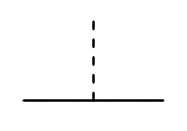
\includegraphics[width=0.2\textwidth]{figs/37a.png}}
  \hfill
  \subfloat[from $V(\psi^\dagger \psi)$, $\propto \lambda = m_h^2/2v^2$]{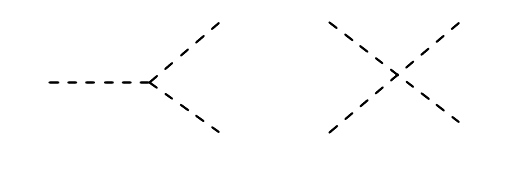
\includegraphics[width=0.4\textwidth]{figs/37b.png}}
  \hfill
  \subfloat[from $(\mathcal{D}_\mu \phi^\dagger)(\mathcal{D}^\mu \phi)$, $\propto g, g^2$]{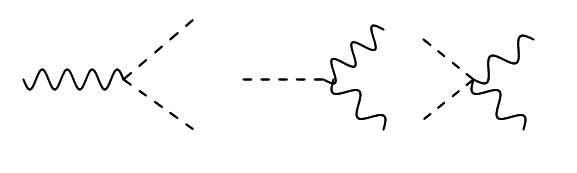
\includegraphics[width=0.4\textwidth]{figs/37c.png}}
\end{figure}
For example, consider interactions between one vector boson and two Goldstone bosons. These come from the term:
\begin{equation}
\mathcal{D}_\mu\chi^\dagger D^\mu \chi = \partial^\mu \chi^\dagger(-ig \underline{W}_\mu \cdot \underline{T} - \frac{ig^\prime}{2} B_\mu) \chi + h.c..
\end{equation}
Considering the neutral current part, 
\begin{equation}
\begin{split}
&igW_\mu^3 \frac{1}{2} \chi^\dagger \tau_3 \partial^\mu \chi + ig^\prime B_\mu \frac{1}{2} \chi^\dagger \partial_\mu \chi + h.c. \\
=\ &ig W_\mu^3(w^\dagger \partial_\mu w - \frac{1}{2} h \partial_\mu h - \frac{1}{2} z \partial_\mu z) + ig^\prime B_\mu (w^\dagger \partial_\mu w + \frac{1}{2} h \partial_\mu h + \frac{1}{2} z \partial_\mu z) + h.c.,
\end{split}
\end{equation}
so for $w^\pm$:
\begin{equation}
\begin{split}
&i(w^\dagger \partial^\mu w - \partial^\mu w^\dagger w)(g W_\mu^3 + g^\prime B_\mu) \\ 
=\ &i(w^\dagger \partial^\mu w)\bigg(g(\cos\theta_w Z_\mu + \sin\theta_w A_\mu) + g^\prime(-\sin\theta_w Z_\mu + \cos\theta_w A_\mu)\bigg) \\
=\ &i(w^\dagger \partial^\mu w)\bigg(g \frac{\cos 2 \theta_w}{\cos\theta_w} Z_\mu + 2e A_\mu \bigg).
\end{split}
\end{equation}
\begin{figure}[!h]
  \centering
  \subfloat[]{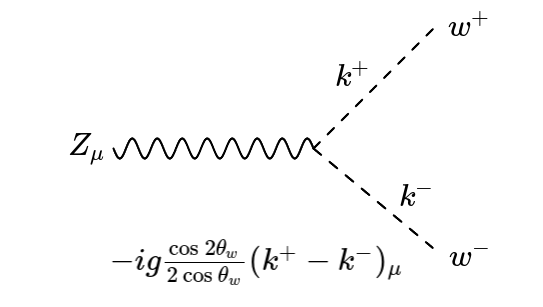
\includegraphics[width=0.5\textwidth]{figs/37d.png}}
  \hfill
  \subfloat[]{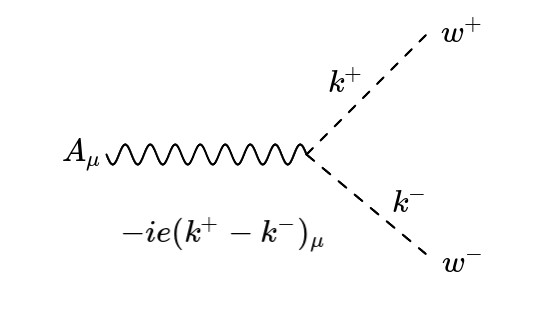
\includegraphics[width=0.5\textwidth]{figs/37e.png}}
\end{figure}
%
\subsubsection{Example: $\bar{\nu} \nu \to W_L^+ W_L^-$ at high energy}
%
There is only one contributing graph at high energy, because the coupling of $w^\pm$ to $\nu e$ is proportional to $m_e$, so we can ignore it. There is also no coupling between the $z$ and $w^+ w^-$, due to custodial symmetry. 
\newline
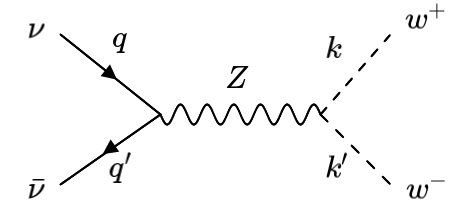
\includegraphics[width=0.5\linewidth]{figs/38a.png}
\newline
\begin{equation}
\begin{split}
\mathcal{M} &= \frac{-ig}{4\cos\theta_w}\bar{v}(q^\prime) \gamma_\mu (1-\gamma^5) u(q) \frac{i}{s-m_Z^2}\bigg(-ig\frac{\cos 2 \theta_w}{2\cos\theta_w}\bigg)(k^\mu - k^{\prime \mu}) \\
&= -ig^2\frac{\cos 2 \theta_w}{4 \cos^2 \theta_w} \frac{\bar{v}(q^\prime)\slashed{k}(1-\gamma^5)u(q)}{s-m_Z^2},
\end{split}
\end{equation}
where we have used that $k+ k^\prime = q + q^\prime$ and $\bar{v}(q^\prime)(\slashed{q} + \slashed{q}^\prime)(1-\gamma^5)u(q)=0$. So
\begin{equation}
\begin{split}
\frac{d\sigma}{d\cos\theta} &\approx \frac{g^2}{32\pi} \frac{\cos^2 2\theta_w}{\cos^4\theta_w} \frac{ut}{4s^3} \qquad \text{at high energy} \\
&= \frac{g^2}{128\pi} \frac{\cos^2 2\theta_w}{\cos^4\theta_w} \frac{1}{16E^2} \sin^2\theta.
\end{split}
\end{equation}
Note that no cancellation is necessary. We can check this by calculating the full result using vector bosons (left as an exercise).
%
\subsubsection{Example: $W_L^+W_L^- \to W_L^+W_L^-$ at high energy}
%
There are two types of graph involving vector bosons: an $s$-channel and a $t$-channel.
\begin{figure}[!h]
  \centering
  \subfloat[$s$-channel]{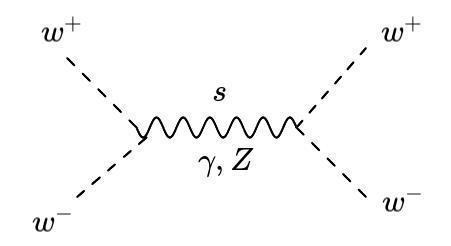
\includegraphics[width=0.5\textwidth]{figs/38b.png}}
  \hfill
  \subfloat[$t$-channel]{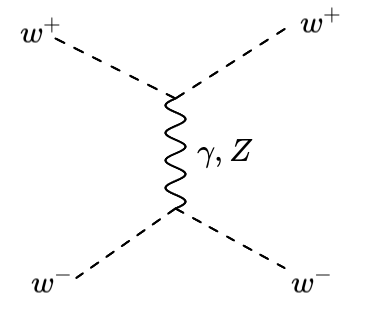
\includegraphics[width=0.3\textwidth]{figs/38c.png}}
\end{figure}
Using $(k^+ + k^-)^2 = 4 m_W^2 -s$, in the $\xi = 1$ gauge we can use the crossing symmetry between the two diagrams to write
\begin{equation}
\begin{split}
\mathcal{M}_{\gamma,Z} &= \bigg( (ie)^2 \frac{i}{s} + (ig)^2 \frac{\cos^2 2\theta_w}{4 \cos^2\theta_w} \frac{i}{s-m_Z^2}\bigg)(4m_w^2-s) + (s \leftrightarrow t) \\
&\approx +\frac{ig^2}{4 \cos^2 \theta_w}\bigg(1 + \cos^2 2\theta_w\frac{m_Z^2}{s-m_Z^2}\bigg)\bigg(1- \frac{4m_w^2}{s}\bigg) + (s \leftrightarrow t) \\
&\approx \frac{ig^2}{2}\frac{m_Z^2}{m_w^2} + \mathcal{O}\bigg(\frac{m_Z^2}{s}\bigg).
\end{split}
\end{equation} 
There are also three pure scalar contributions: a quartic vertex and two Higgs graphs.
\newline
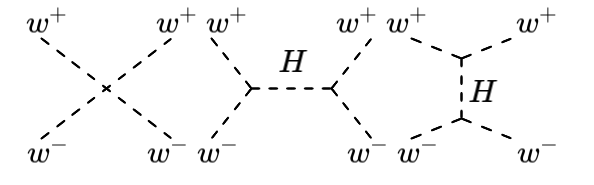
\includegraphics[width=\linewidth]{figs/38d.png}
\newline
These have contributions
\begin{equation}
\begin{split}
\mathcal{M}_h &= -4i\lambda + (-2i\lambda v)^2 \bigg(\frac{i}{s-m_h^2} + \frac{i}{t-m_h^2}\bigg) \\
&=-\frac{ig^2}{4}\frac{m_h^2}{m_w^2}\bigg(\frac{s}{s-m_h^2} + \frac{t}{t-m_h^2}\bigg) \\
&\approx - \frac{ig^2}{2}\frac{m_h^2}{m_w^2} + \mathcal{O}\bigg(\frac{m_h^2}{s}\bigg),
\end{split}
\end{equation}
where we have used the fact that $\lambda = g^2m_h^2/8m_w^2$, $v=2m_w/g$. So the high energy behaviour is controlled (in part) by the Higgs:
\begin{equation}
\mathcal{M} \approx -\frac{ig^2}{2}\frac{m_Z^2-m_h^2}{m_w^2} + \mathcal{O}\bigg(\frac{m^2}{s}\bigg).
\end{equation}
Note that if the Higgs were very heavy, $m_h^2 \gg m_w^2$, and unitarity would be violated:
\begin{equation}
\frac{d\sigma}{d\Omega} \approx \frac{1}{64\pi^2}\frac{g^4}{4}\frac{m_h^4}{m_W^4}\frac{1}{s},
\end{equation}
so 
\begin{equation}
\sigma \approx \frac{G_F^2 m_h^4}{2\pi s} \leq \frac{16 \pi}{s},
\end{equation}
so, considering $\sigma =1$,
\begin{equation}
m_h^2 \leq \frac{4 \sqrt{2} \pi}{G_F},
\end{equation}
i.e. $m_h \leq 1$ TeV.
%
\subsection{Summary}
%
\begin{equation}
\mathcal{L} = \mathcal{L}_D + \mathcal{L}_{YM} + \mathcal{L}_{Y} + \mathcal{L}_h + \mathcal{L}_{\text{gauge fixing}}
\end{equation}
IN the unitary gauge, the Goldstone bosons disappear, but renormalisability is not manifest. So for high energy behaviour it is better to work in the $R_\xi$ gauge. 
\subsubsection{Parameter counting}
\begin{table}[h!]
\begin{tabular}{l|l|l}
\centering
$\mathcal{L}_D$ & $\alpha, \alpha_s, \theta_w$ & 3 parameters: "SU(3)$\otimes$SU(2)$\otimes$U(1)" $\implies$ GUT? \\ \hline
$\mathcal{L}_{YM}$  &                                                                       
& no extra parameters\\ \hline
$\mathcal{L}_h$    &                                                                       $m_W, m_h$ & 2 parameters (are they related?)  \\ \hline
$\mathcal{L}_{Y, \text{lep}}$  &                                                                           $m_e, m_\mu, m_\tau$ & 3 parameters (not understood?) \\ \hline
$\mathcal{L}_{Y, \text{quark}}$ &                                                                           $u, d, s, c, b, t$ + 3 angles + 1 phase & 10 parameters  \\ \hline
$\mathcal{L}_{Y, \nu}$ & 3 masses + 3 angles + 3 phases                                                              &  9 parameters                  
\end{tabular}
\end{table}
